\documentclass[10pt,twocolumn]{article}
\usepackage[utf8]{inputenc}
\usepackage[T1]{fontenc}
\usepackage[spanish,es-nodecimaldot]{babel}
\addto\captionsspanish{\renewcommand{\tablename}{Tabla}}
\usepackage{amsmath,amssymb,graphicx,booktabs,geometry,caption,lmodern,microtype,hyperref,xcolor,stfloats}
\geometry{a4paper,margin=1.35cm,columnsep=0.55cm}
\usepackage{titlesec}
\titlespacing*{\section}{0pt}{4pt}{1.5pt}
\titlespacing*{\subsection}{0pt}{3pt}{1pt}
\setlength{\parindent}{0pt}\setlength{\parskip}{2pt}
\captionsetup{font=footnotesize,labelfont=bf,skip=3pt}
\definecolor{accent}{HTML}{174A6E}
\hypersetup{colorlinks=true,linkcolor=accent,urlcolor=accent,citecolor=accent,pdftitle={Test de Circuitos Integrados: Fallos Stuck-At, Stuck-Open y Arquitectura Scan Path},pdfauthor={Leonardo Sait Yactayo Tolentino; Marco Antonio Arcila Santander}}
\setlength{\textfloatsep}{5pt plus 1pt minus 1pt}
\setlength{\dbltextfloatsep}{5pt plus 1pt minus 1pt}
\setlength{\intextsep}{5pt plus 1pt minus 1pt}

\title{\vspace{-12pt}\textbf{\large Test de Circuitos Integrados: Fallos Stuck-At, Stuck-Open y Arquitectura Scan Path}\texorpdfstring{\\[2pt]}{ -- }
\normalsize Laboratorio Dirigido N.º 04 -- Microelectrónica y Sistemas Nanoelectrónicos}
\author{\small\textbf{Leonardo Sait Yactayo Tolentino} (23190214) \quad \textbf{Marco Antonio Arcila Santander} (23190140)\texorpdfstring{\\}{, }
\footnotesize Facultad de Ingeniería Electrónica y Eléctrica -- Universidad Nacional Mayor de San Marcos\texorpdfstring{\\}{, }
\footnotesize \textit{Docente: MsC. Luz Antuanet Adanaqué Infante} \quad | \quad Semestre 2026-II\vspace{-8pt}}
\date{}

\begin{document}
\renewcommand{\tablename}{Tabla}
\maketitle
\vspace{-10pt}

\section{Introducción y Metodología}
En el presente informe técnico, dirigido a nuestra profesora MsC.\ Luz Antuanet Adanaqué Infante, caracterizamos analíticamente y validamos mediante simulación SPICE en LTspice las metodologías de test estructural en circuitos integrados digitales: el modelo de fallo por adhesión (\emph{stuck-at}), el defecto en circuito abierto (\emph{stuck-open}) y el diseño orientado al test mediante camino de exploración (\emph{Scan Path})~\cite{guia,bushnell}.

Utilizamos la biblioteca \texttt{cmos035\_cells.lib} (MOS nivel~1 de $0{,}35\,\mu\mathrm{m}$, $V_{DD}=3{,}3\,\mathrm{V}$) y umbral lógico $V_{th}=V_{DD}/2=1{,}65\,\mathrm{V}$ ($V>1{,}65\,\mathrm{V} \Rightarrow 1$). Todas las mediciones escalares fueron verificadas directamente entre los archivos \texttt{.log} y sus trazas \texttt{.raw} originales (521/521 mediciones coincidentes), diferenciando explícitamente las lecturas de cursores gráficos, las muestras puntuales \texttt{.meas} y los extremos transitorios reconstruidos del archivo \texttt{.raw}.

\section{Bloque Combinacional: ATPG y Fallos}
\subsection{Circuito Sano y Nudos de Test}
Evaluamos el segmento $f$ del decodificador BCD a 7 segmentos, $Y = d + c\,\overline{b\,a} + \overline{b+a}$ (compuertas NAND2, NOR2, AND2 y OR3). Las entradas $b$ y $a$ presentan \emph{fan-out} $=2$: $b$ se ramifica hacia NAND2 (nudo~3) y NOR2 (nudo~5), y $a$ hacia NAND2 (nudo~4) y NOR2 (nudo~6), generando 10 nudos de test y 20 fallos \emph{stuck-at} únicos.

Al aplicar los 16 vectores $d\,c\,b\,a$ en el circuito sano (\texttt{NUDO=0}), obtuvimos en \texttt{P1\_segf\_stuckat.log} la secuencia lógica \texttt{1000111011111111}, coincidente en 16/16 posiciones con la tabla teórica ($Y=1$ en los dígitos BCD $\{0,4,5,6,8,9\}$). Para el vector $0001$, medimos con cursores gráficos el cruce por $1{,}65\,\mathrm{V}$ en $t_{V(a)}=10{,}050029\,\mathrm{ns}$ y $t_{V(y)}=10{,}088119\,\mathrm{ns}$, resultando $t_{pHL}=38{,}090\,\mathrm{ps}\approx 38{,}1\,\mathrm{ps}$ (lectura de cursores gráficos, no directiva \texttt{.meas}).

\begin{figure}[t]
\centering
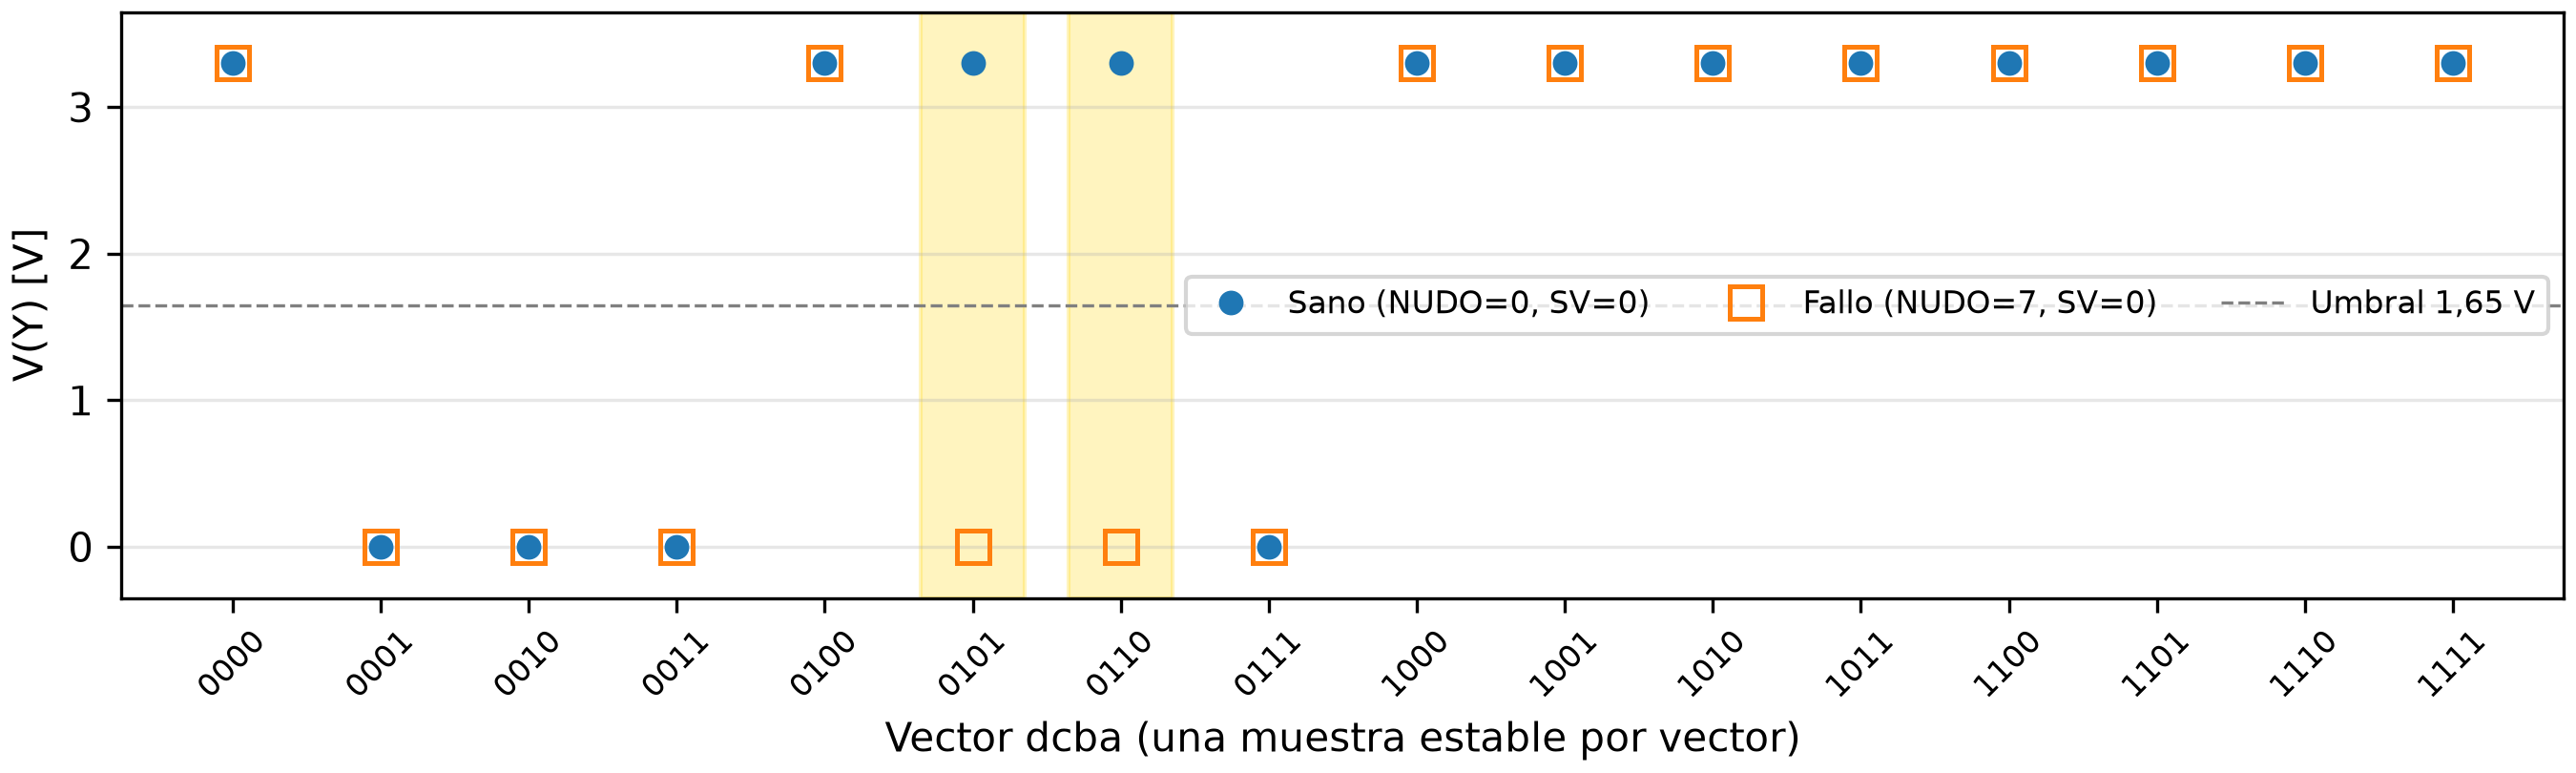
\includegraphics[width=\linewidth]{../figuras/stuckat_muestras.png}
\caption{Muestras discretas \texttt{.meas} (\texttt{v00}--\texttt{v15}) de $V(Y)$ extraídas de \texttt{P1\_segf\_stuckat.log}: circuito sano (\texttt{NUDO=0, SV=0}) frente a fallo $7/\text{s-a-0}$ (\texttt{NUDO=7, SV=0}), con divergencia únicamente en $0101$ y $0110$. \emph{Nota:} Gráfica generada en Python a partir de muestras discretas del registro, no captura continua de LTspice.}
\label{fig:stuckat}
\end{figure}

\subsection{D-Algoritmo, Diccionario y Cobertura}
Mediante el algoritmo D de Roth~\cite{bushnell} derivamos los vectores detectores de los seis casos requeridos (nudos 7, 5 y 9 para \emph{s-a-0} y \emph{s-a-1}), validando cada predicción contra las corridas correspondientes de \texttt{P1\_segf\_stuckat.log}. Al contrastar las 140 respuestas de los 20 fallos frente al conjunto de 7 vectores optimizados (\texttt{0101, 0111, 0000, 0001, 0010, 0110, 1010}), comprobamos coincidencia del 100\,\% con el log (véase Fig.~\ref{fig:stuckat}).

Corregimos el doble conteo detectado en la hoja preliminar sobre $10/\text{s-a-0}$: la progresión acumulada de fallos únicos es 5 (25\,\%), 12 (60\,\%), 15 (75\,\%), 17 (85\,\%), 18 (90\,\%), 19 (95\,\%) y 20 (100\,\%), siendo indispensable el 7.º vector (\texttt{1010}) para detectar $1/\text{s-a-0}$. En comparación, el conjunto funcional BCD (\texttt{0000--1001}) requiere 10 vectores para alcanzar el 100\,\%, mientras que el conjunto aleatorio de 4 vectores (\texttt{1100, 0011, 1001, 0110}) detecta solo 10/20 fallos (50\,\%).

\subsection{Fallo Stuck-Open y Transitorios}
En \texttt{P1\_stuckopen.cir}, la resistencia $R_{SO}$ ($1\,\mathrm{m}\Omega$ sano; $1\,\mathrm{T}\Omega$ abierto) desconecta el drenaje del NMOS de entrada $a$ en \texttt{NOR2\_SO}. Ante la secuencia $T_0(0000)\to T_1(0001)\to T_2(0011)\to T_3(0001)$ (Fig.~\ref{fig:open}), en $T_1$ el nodo interno $o8$ queda flotante tras haberse precargado en $T_0$ a $3{,}30\,\mathrm{V}$, manteniendo $Y=1$ frente a $Y=0$ del circuito sano (detección). En $T_2$ ($b=1$), el NMOS sano de $b$ descarga $o8$ a $0\,\mathrm{V}$, por lo que al retornar a $0001$ en $T_3$, $o8$ flota descargado ($Y=0$) y el fallo pasa inadvertido. Por ello hacen falta \textbf{2 vectores en pareja ordenada} ($0000\to 0001$); el conjunto optimizado de 7 vectores sí detecta este defecto porque su 3.º (\texttt{0000}) y 4.º vector (\texttt{0001}) son consecutivos en ese orden.

En \texttt{P1\_stuckopen.raw} distinguimos las muestras \texttt{.meas} estables ($t=8,18,28,38\,\mathrm{ns}$) de los extremos transitorios: en $T_1$, $V(o8)$ alcanza un máximo de $3{,}451\,\mathrm{V}$ a $10{,}120\,\mathrm{ns}$ y permanece en $3{,}450976\,\mathrm{V}$ a $18\,\mathrm{ns}$; en $T_2$ presenta un pico inicial de $3{,}811\,\mathrm{V}$ a $20{,}045\,\mathrm{ns}$ antes de descargarse a $0{,}00\,\mathrm{V}$; y en $T_3$ alcanza un mínimo de $-0{,}144\,\mathrm{V}$ a $30{,}100\,\mathrm{ns}$ que relaja a $-0{,}114028\,\mathrm{V}$ a $38\,\mathrm{ns}$. Estos sobreimpulsos fuera de $[0;\,3{,}3]\,\mathrm{V}$ son coherentes con el acoplamiento capacitivo (\emph{feedthrough}) vía capacidades de solapamiento sobre el nudo de alta impedancia al conmutar $a$ y $b$.

\begin{figure}[t]
\centering
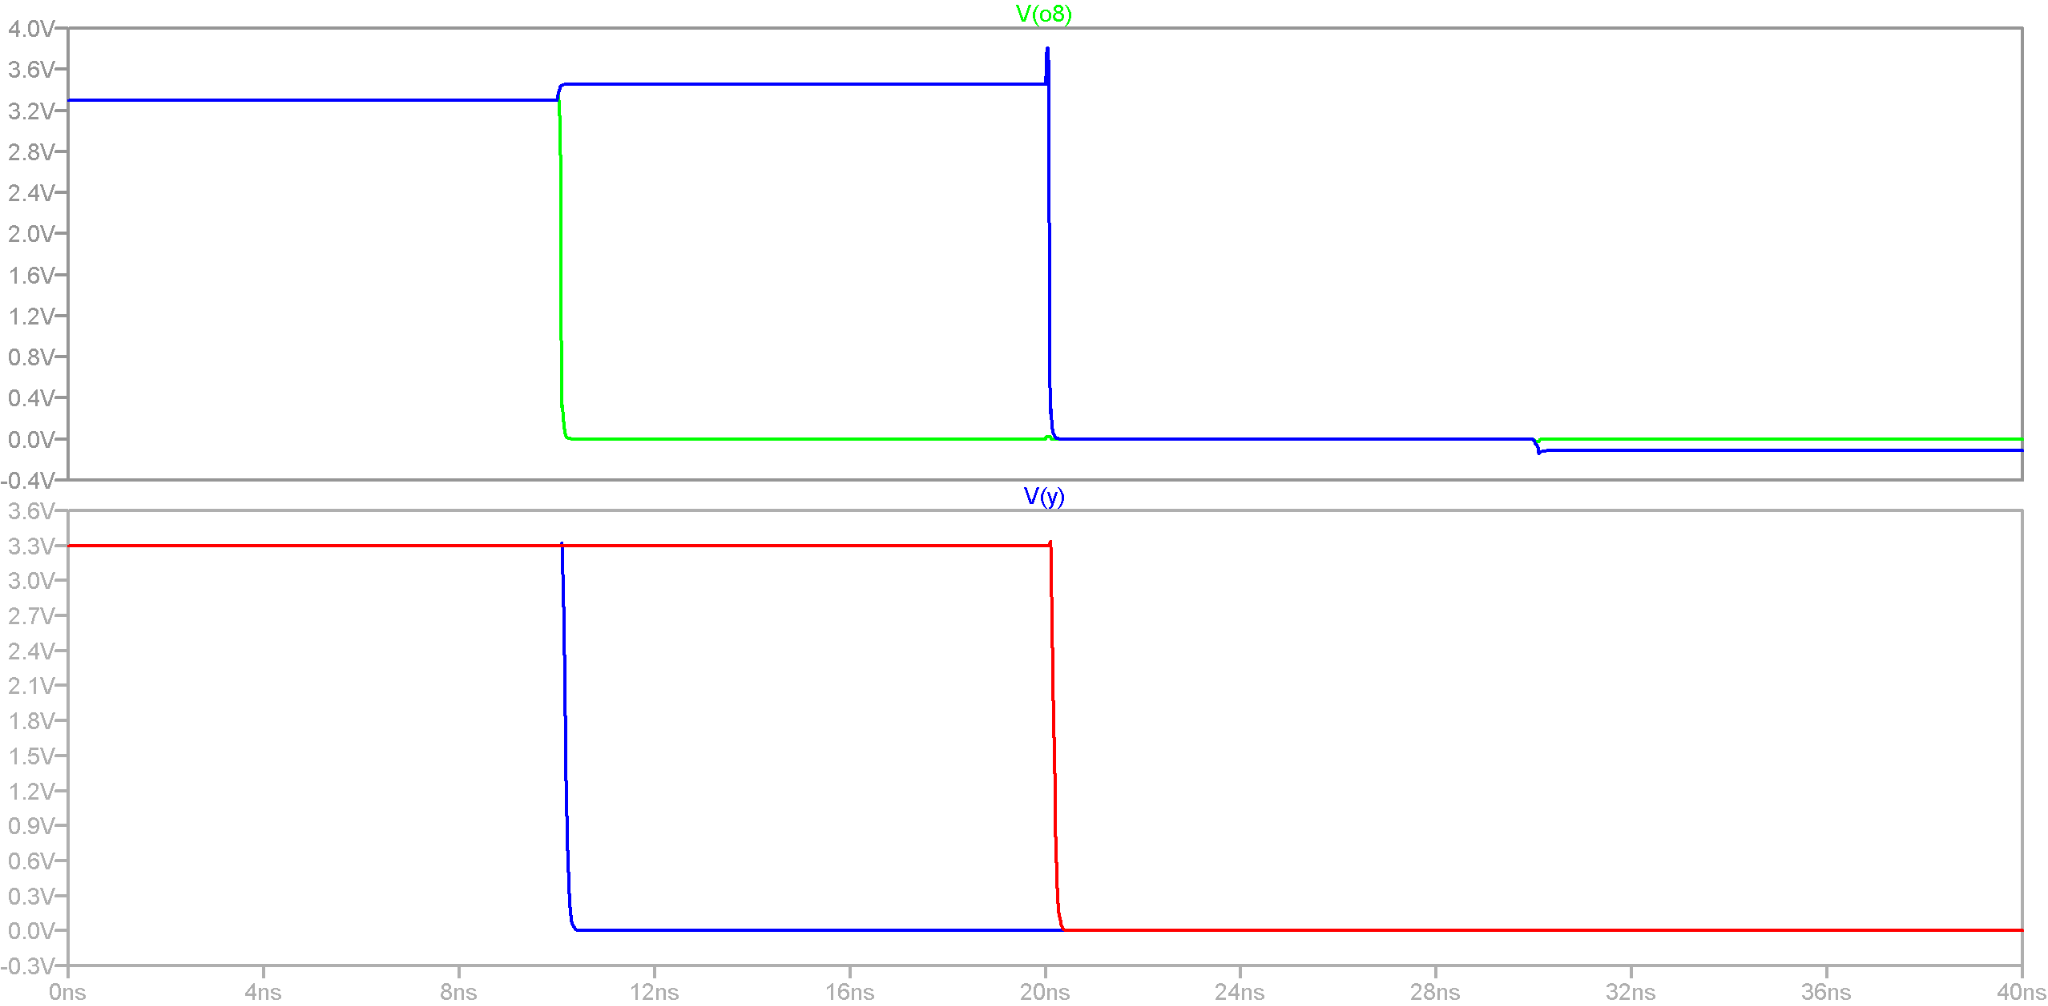
\includegraphics[width=\linewidth]{../figuras/stuckopen.png}
\caption{Formas de onda históricas de LTspice del ensayo \emph{stuck-open} (\texttt{P1\_stuckopen.cir}, secuencia $T_0\dots T_3$). Panel superior $V(o8)$: traza \textbf{verde} = sano ($R_{SO}=1\,\mathrm{m}\Omega$) y \textbf{azul} = fallo ($R_{SO}=1\,\mathrm{T}\Omega$). Panel inferior $V(y)$: \textbf{azul} = sano y \textbf{rojo} = fallo. Captura original de los autores.}
\label{fig:open}
\end{figure}

\section{Lógica Secuencial y Scan Path}
\subsection{Modo Funcional y Test de Flush}
El contador síncrono de 3 bits con habilitación $E$ emplea 3 biestables SDFF, 3 XOR2 y 3 AND2. En modo funcional (\texttt{P2\_func.log}, $SE=0$, $T_{CLK}=20\,\mathrm{ns}$), las 10 muestras verifican que $Z=E\cdot Q_2Q_1Q_0$ se activa por primera vez en el ciclo $k=7$ ($149\,\mathrm{ns}$). Para $N$ bits desde $0$, el primer $Z=1$ exige $K=2^N-1$ ciclos; para $N=20$ a $50\,\mathrm{MHz}$ se requieren $(2^{20}-1)\cdot 20\,\mathrm{ns}=20{,}9715\,\mathrm{ms}$ frente a $400\,\mathrm{ns}$ mediante precarga por \emph{scan}.

En el \emph{flush test} ($SE=1$), verificamos $SO[k]=SI[k-3]$ sobre la cadena $SI\to FF0\to FF1\to FF2\to SO$ ($1101001000000 \mapsto 0001101001000$, retardo de 3 ciclos). Un fallo \emph{s-a-0} en cualquier biestable produce ceros permanentes en $SO$ desde $k=3$ (detecta sin localizar); un fallo \emph{s-a-1} entrega unos continuos con retardos discriminables: 0 ciclos en $FF2$ ($k=0$), 1 ciclo en $FF1$ ($k=1$) y 2 ciclos en $FF0$ ($k=2$). Documentamos que \texttt{P2\_flush.log} (\texttt{method=gear}) y \texttt{P2\_flush\_fix.log} (\texttt{cshunt=2f}) abortaron por convergencia ($>350$ y $411$ avisos), respaldando la tabla únicamente en \texttt{P2\_flush\_fix2.log} ($6{,}334\,\mathrm{s}$, 0 avisos) con las opciones numéricas \texttt{cshunt=20f gshunt=1n reltol=0.01 trtol=7 vntol=1m abstol=1n itl4=500}.

\subsection{Programa Scan, Glitch de $Z$ y Diagnóstico}
Ejecutamos el programa oficial de 5 vectores ($V_1=001/0$, $V_2=110/1$, $V_3=011/1$, $V_4=001/1$, $V_5=111/1$), totalizando $N=3+4(5)=23$ ciclos ($0{,}46\,\mu\mathrm{s}$ a $50\,\mathrm{MHz}$, Fig.~\ref{fig:scan}). En la captura de $V_3$ ($011\to 100$ tras el flanco a $230\,\mathrm{ns}$), $Q_2$ sube a 1 antes de que la extinción de $g_2=E\cdot Q_0\cdot Q_1$ atraviese la lógica AND, produciendo un riesgo estático-0 en $Z=g_2\cdot Q_2$. En \texttt{P2\_scan.raw} medimos un pico de $2{,}1694\,\mathrm{V}$ en $t=230{,}700\,\mathrm{ns}$, con ancho por encima del umbral lógico ($1{,}65\,\mathrm{V}$) de $0{,}134\,\mathrm{ns}$ y ancho a media altura (FWHM a $1{,}0847\,\mathrm{V}$) de $0{,}210\,\mathrm{ns}$. Cabe precisar que \texttt{P2\_scan.cir} usa las mismas directivas \texttt{.options} de estabilización numérica que \texttt{P2\_flush\_fix2.cir}; estas son parámetros del simulador (no elementos físicos del CI) que atenúan y redondean parcialmente la amplitud del pulso transitorio. No afecta el test porque \texttt{z\_v3} se muestrea en $229\,\mathrm{ns}$, $1\,\mathrm{ns}$ antes del flanco en régimen estático ($V(z)\approx 0\,\mathrm{V}$).

\begin{figure}[t]
\centering
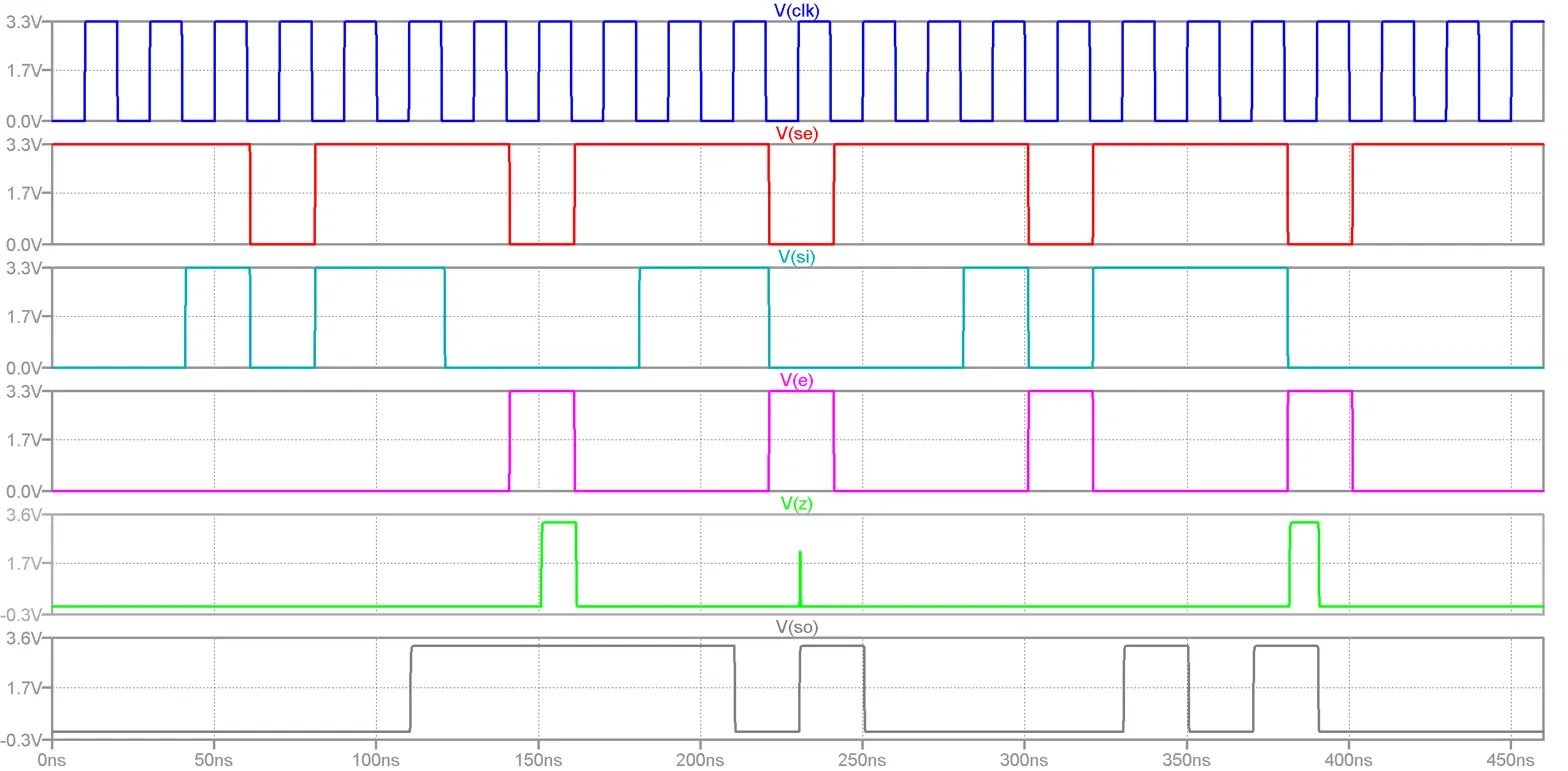
\includegraphics[width=\linewidth]{../figuras/scan.png}
\caption{Captura histórica de LTspice para el programa \emph{scan} sano (\texttt{P2\_scan.cir}, \texttt{FAULT=0}, 23 ciclos a $50\,\mathrm{MHz}$, muestreo $1\,\mathrm{ns}$ antes de cada flanco). Canales de arriba hacia abajo: $V(\mathrm{clk})$ azul, $V(\mathrm{se})$ rojo, $V(\mathrm{si})$ cian, $V(\mathrm{e})$ magenta, $V(\mathrm{z})$ verde (con $Z=1$ en $V_2, V_5$ y pico espurio en $V_3$) y $V(\mathrm{so})$ gris.}
\label{fig:scan}
\end{figure}

En las 25 combinaciones de diagnóstico (\texttt{P2\_scan.log}, \texttt{FAULT=0..4}), todos los fallos se detectan por $SO$ (0\,\% por $Z$), con primeros detectores F1$\to V_3$, F2$\to V_4$, F3$\to V_2$ y F4$\to V_1$. Por el D-algoritmo, F2 ($Q_1\to\text{AND}$ \emph{s-a-1}) exige $Q_1=0$ y $g_1=E\cdot Q_0=1$, restringiendo el detector a $X01/1$: solo $V_4=001/1$ lo satisface. Para 32 biestables y 500 vectores, dividir 1 cadena ($16\,532$ ciclos, $330{,}64\,\mu\mathrm{s}$, 3 pads) en 4 cadenas paralelas de 8 ($4\,508$ ciclos, $90{,}16\,\mu\mathrm{s}$, 1 pad $SE$ + 4 $SI$ + 4 $SO$ = 9 pads) acelera $3{,}67\times$ el test al costo de \textbf{6 pads adicionales}.

En sección aparte (\texttt{ensayo\_26/P2\_scan.log}) verificamos el conjunto alternativo con $V_{4,\text{exp}}=101/1$: las 25 respuestas coinciden y vuelven a F2 observable también en $Z$. Sobre los 16 nudos (32 fallos \emph{stuck-at}) del núcleo combinacional en \texttt{P2\_counter\_core.inc}, demostramos por enumeración exhaustiva (1820 combinaciones) que 4 vectores alcanzan como máximo 31/32 fallos, pues existen 5 conjuntos disjuntos exigidos cada uno por un fallo único: $S_1=\{111/1\}$, $S_2=\{011/1\}$, $S_3=\{001/1,101/1\}$, $S_4=\{xx0/1\}$ y $S_5=\{xx1/0\}$ (en LTspice solo se inyectan \texttt{FAULT=1..4}).

\section{Respuestas a las Preguntas de la Guía}
\textbf{1. Nudos de test y fan-out:} Las bifurcaciones de $b$ hacia NAND2 (nudo~3) y NOR2 (nudo~5) pueden sufrir defectos independientes en vías o pistas metálicas; por ello cada entrada de celda es un nudo de test separado y no basta el nudo topológico global. \textbf{2. Defecto físico vs.\ stuck-at:} Un \emph{s-a-0} en entrada de NAND2 equivale a un cortocircuito de baja resistencia hacia $V_{SS}$ (o ruptura de puerta/canal acoplada a masa); un \emph{s-a-1} modela un corto hacia $V_{DD}$. Defectos resistivos o de óxido pueden causar además retardos anómalos. \textbf{3. Saturación de cobertura:} Los primeros vectores cubren fallos de alta observabilidad (60\,\% en 2 vectores); los restantes requieren rutas específicas y justifican el flujo industrial de vectores aleatorios seguidos de simulación de fallos y ATPG determinista. \textbf{4. Conjuntos funcionales:} El BCD cubre 100\,\% aquí por ser un circuito combinacional mínimo sin redundancia; en sistemas secuenciales grandes las secuencias funcionales dejan estados profundos sin excitar ni observar. \textbf{5. Redundancia y glitch:} Añadir una AND3 ($\overline{c}\,\overline{b}\,\overline{a}$) a la OR3 deja su salida \emph{s-a-0} indetectable: activarla exige $0000$, vector bajo el cual NOR2 también entrega 1 (valor controlante de OR3), enmascarando el error $D$; los riesgos deben resolverse mediante diseño síncrono~\cite{pollan}. \textbf{6. Orden de vectores:} El \emph{stuck-open} convierte la capacidad del nodo flotante en memoria dinámica dependiente del estado previo, exigiendo parejas ordenadas ($0000\to 0001$), a diferencia del \emph{stuck-at} estático. \textbf{7. Orden de carga en scan:} En $SI\to FF0\to FF1\to FF2\to SO$, el primer bit en entrar termina en $FF2$, cargándose en orden $Q_2, Q_1, Q_0$; al invertir la cadena a $SI\to FF2\to FF1\to FF0\to SO$, se cargaría primero $Q_0$. \textbf{8. Reset asíncrono:} Fija el estado inicial conocido ($000$) tras el encendido, evitando estados indeterminados ($X$) tanto en la convergencia SPICE como en los primeros ciclos en $SO$ del chip real. \textbf{9. Sobrecosto del scan:} En \texttt{cmos035\_cells.lib}, cada celda \texttt{SDFF} consta de 4 inversores (8 MOS), 6 puertas de transmisión (12 MOS) y 2 compuertas NOR2 (8 MOS), sumando \textbf{28 transistores} (núcleo total: $3\times 12 + 3\times 6 + 3\times 28 = 138$ transistores, más 8 de buffers). El multiplexor de scan añade área y retardo en la ruta funcional de $D$ más 3 pads dedicados, pero reduce el test de complejidad exponencial $O(2^N)$ a lineal $O(N)$. \textbf{10. Boundary Scan (JTAG):} La norma IEEE~1149.1 coloca celdas bidireccionales en los pines mediante 4 terminales (\texttt{TDI, TDO, TCK, TMS}) para probar pistas e interconexiones en PCB (\texttt{EXTEST}) y el núcleo (\texttt{INTEST}); reduce significativamente la dependencia de \emph{fixtures} físicos (camas de agujas) en pruebas de interconexión digital, aunque no elimina toda necesidad de acceso físico ni sustituye las pruebas eléctricas analógicas o de alta velocidad.

\section{Conclusiones}
1. Validamos el 100\,\% de las 521 mediciones escalares entre registros \texttt{.log} y trazas \texttt{.raw}, corrigiendo la progresión de cobertura a 7 vectores únicos (25\,\% a 100\,\%) y demostrando la necesidad de parejas ordenadas ($0000\to 0001$) para defectos \emph{stuck-open}.\\
2. Comprobamos la integridad de la cadena \emph{scan} mediante el \emph{flush} de 3 ciclos (\texttt{P2\_flush\_fix2.log}), la discriminación unívoca de \emph{s-a-1} por latencia (0, 1 y 2 ciclos) y el diagnóstico del 100\,\% de los fallos inyectados en el programa oficial ($V_4=001/1$).\\
3. Caracterizamos en \texttt{P2\_scan.raw} el riesgo estático-0 de $Z$ en $V_3$ ($2{,}1694\,\mathrm{V}$ pico; $0{,}134\,\mathrm{ns}$ sobre $1{,}65\,\mathrm{V}$; $0{,}210\,\mathrm{ns}$ FWHM), confirmando su inocuidad frente al muestreo estático a $229\,\mathrm{ns}$ y demostrando formalmente por qué 4 vectores no cubren los 32 fallos del núcleo combinacional.

\begin{thebibliography}{9}\footnotesize
\bibitem{guia} MsC.\ L.\ A.\ Adanaqué Infante, \emph{Guía de Laboratorio: Test de Circuitos Integrados (Stuck-at y Scan Path)}, LD4, FIEE-UNMSM, 2026-II.
\bibitem{bushnell} M.\ L.\ Bushnell y V.\ D.\ Agrawal, \emph{Essentials of Electronic Testing for Digital, Memory and Mixed-Signal VLSI Circuits}, Kluwer/Springer, 2000.
\bibitem{pollan} T.\ Pollán Santamaría, \emph{Tecnología Electrónica}, cap.\ 25 «Test de circuitos integrados», Univ.\ de Zaragoza.
\end{thebibliography}

\end{document}
